\documentclass[12pt,a4]{article}
\usepackage{physics, amsmath,amsfonts,amsthm,amssymb, mathtools,steinmetz, gensymb, siunitx}	% LOADS USEFUL MATH STUFF
\usepackage{xcolor,graphicx}
\usepackage{caption}
\usepackage{subcaption}
\usepackage[left=45pt, top=20pt, right=45pt, bottom=45pt ,a4paper]{geometry} 				% ADJUSTS PAGE
\usepackage{setspace}
\usepackage{tikz}
\usepackage{pgf,tikz,pgfplots,wrapfig}
\usepackage{mathrsfs}
\usepackage{fancyhdr}
\usepackage{float}
\usepackage{array}
\usepackage{booktabs,multirow}
\usepackage{bm}
\usepackage{tensor}
\usepackage{listings}
 \lstset{
    basicstyle=\ttfamily\small,
    numberstyle=\footnotesize,
    numbers=left,
    backgroundcolor=\color{gray!10},
    frame=single,
    tabsize=2,
    rulecolor=\color{black!30},
    title=\lstname,
    escapeinside={\%*}{*)},
    breaklines=true,
    breakatwhitespace=true,
    framextopmargin=2pt,
    framexbottommargin=2pt,
    inputencoding=utf8,
    extendedchars=true,
    literate={á}{{$\rho$}}1 {ã}{{\~a}}1 {é}{{\'e}}1,
}
\DeclareMathOperator{\sign}{sgn}

\usetikzlibrary{decorations.text, calc}
\pgfplotsset{compat=1.7}

\usetikzlibrary{decorations.pathreplacing,decorations.markings}
\usepgfplotslibrary{fillbetween}

\newcommand{\vect}[1]{\boldsymbol{#1}}

\usepackage{hyperref}

%\usepackage[style= ACM-Reference-Format, maxbibnames=6, minnames=1,maxnames = 1]{biblatex}
%\addbibresource{references.bib}


\hypersetup{pdfborder={0 0 0},colorlinks=true,linkcolor=black,urlcolor=cyan,}
\allowdisplaybreaks
%\hypersetup{
%
%    colorlinks=true,
%
%    linkcolor=blue,
%
%    filecolor=magenta,      
%
%    urlcolor=cyan,
%
%    pdftitle={An Example},
%
%    pdfpagemode=FullScreen,
%
%    }
%}

\title{
\textsc{Statistical Physics Homework 1}
}
\author{\textsc{J L Gouws}
}
\date{\today
\\[1cm]}



\usepackage{graphicx}
\usepackage{array}




\begin{document}
\thispagestyle{empty}

\maketitle

\begin{enumerate}
  \item
    \begin{enumerate}
      \item
        Taylor expanding the pressure $P(T, v)$ about the equilibrium point up to third order (and ignoring the order term to save space) gives:
        \begin{equation*}
          P (T, v) = P(T, v_c) + \frac{\partial P}{\partial v}\left(T, v_c\right)(v - v_c)  + \frac{1}{2}\frac{\partial^2 P}{\partial v^2}\left(T, v_c\right)(v - v_c)^2  + \frac{1}{6}\frac{\partial^3 P}{\partial v^3}\left(T, v_c\right)(v - v_c)^3
          % = \left. P(T, v_c) + \frac{\partial P}{\partial v}\left(T, v_c\right)(v - v_c)  + \frac{\partial^2 P}{\partial v^2}\left(T, v_c\right)(v - v_c)^2  + \frac{\partial^3 P}{\partial v^3}\left(T, v_c\right)(v - v_c)^3\right|_{v=v_g}
        \end{equation*}
        Equating $P(T, v_l) = P(T, v_g)$, noting $v_l - v_c = -x$ and $v_g - v_c = y$, yields:
        \begin{align*}
          P(T, v_c) - a x  + b x^2  - c x^3 = P(T, v_c) + a y  + b y^2  + c y^3
        \end{align*}
        Rearranging gives:
        \begin{align}
          a (x + y)  + b ( y^2 - x^2)  + c (x^3 + y ^3) = 0 \label{eq:ChemEquiEquality1}
        \end{align}
        And for the condition:
        \begin{equation*}
          g_{v_l} = g_{v_g}
        \end{equation*}
        Using the formula:
        \begin{equation*}
          g(T, v) = A (T) + P(T, v) v - \int_1 ^v P dv
        \end{equation*}
        to calculate $g_{v_l}$ to fourth order in ``$\Delta v$'':
        \begin{align*}
          g(T, v_l) &= A(T) + \left(P(T, v_c) - a x + b x^2 - c x^3\right)(1 - x) - \int_1^{(1-x)} P(T, v_c) + a (v - v_c) \\
                    & \quad + b(v - v_c)^2  + c (v - v_c)^3 dv\\
                    &= A(T) + \left(P(T, v_c) - a x + b x^2 - c x^3\right)(1 - x) \\
                    & \quad - \left[ P(T, v_c)v + a \frac{(v - v_c)^2}{2} + \frac{b(v - v_c)^3}{3}  + \frac{c (v - v_c)^4}{4}\right]_1^{(1-x)}\\
                    &= A(T) + P(T, v_c) - P(T, v_c) x - a x + b x^2 - c x^3 + a x^2 - b x^3 + c x^4 \\
                    & \quad - P(T, v_c) + P(T, v_c) x - a \frac{x^2}{2} + \frac{bx^3}{3} - \frac{c x^4}{4} + P(T, v_c)\\
                    &= A(T) + P(T, v_c) - a x + (b + a / 2) x^2 - (c + 2 b / 3) x^3 + \frac{3 c x^4}{4}
        \end{align*}
        Simiarly for $v_g$, the calculation is $x \to -y$:
        \begin{align*}
          g(T, v_g) &= A(T) + P(T, v_c) + a y + (b + a / 2) y^2 - (c + 2 b / 3) y^3 + \frac{3 c y^4}{4}
        \end{align*}
        Equating these and dropping the fourth order terms results in:
        \begin{align}
          a (x + y)  + (b + a / 2) ( y^2 - x^2)  + (c + 2 b / 3) (x^3 + y ^3) = 0 \label{eq:ChemEquiEquality2}
        \end{align}
      \item
        Taking Eq.~\ref{eq:ChemEquiEquality2} and subtracting Eq.~\ref{eq:ChemEquiEquality1} gives:
        \begin{equation*}
          \frac{a}{2}(y^2 - x^2) + \frac{2 b}{3} (x^3 + y^3) = 0 \Rightarrow 3 a(y^2 - x^2) + 4 b (x^3 + y^3) = 0
        \end{equation*}
        Factorizing the terms:
        \begin{align*}
                      &3 a(y^2 - x^2) + 4 b (x^3 + y^3) = 0\\
          \Rightarrow &3 a(y - x)(x + y) + 4 b (x + y) (x^2  - xy + y^2) = 0\\
          \Rightarrow &(x + y)(3 a (y - x) + 4 b (x^2  - xy + y^2)) = 0
        \end{align*}
        One algebraic solution is:
        \begin{equation*}
          x + y = 0
        \end{equation*}
        Which is breaks the assumption $x, y \geq 0$, the other solutions are given by:
        \begin{equation*}
          3 a (y - x) + 4 b (x^2  - xy + y^2) = 0
        \end{equation*}
        This is a quadratic equation in $x$ and $y$:
        \begin{equation*}
          y^2 + (3a/4b - x)y + x^2 - 3a x/4b = 0
        \end{equation*}
        This has solutions:
        \begin{align*}
          y &= \frac{1}{2}\left(x - 3a / 4b \pm \sqrt{(3a/4b - x)^2 - 4 (x^2 - 3a x / 4b)} \right)\\
            &= \frac{1}{2}\left(x - 3a / 4b \pm \sqrt{(3a/4b)^2 + 3a x / 2b - 3x^2} \right)
        \end{align*}
        And expanding the square root about the constant term:
        \begin{align*}
          y &= \frac{1}{2}\left(x - 3a / 4b \pm \left(\sqrt{(3a/4b)^2 } + \frac{1}{2}\frac{1}{\sqrt{(3a/4b)^2 }}( 3a x / 2b ) + o (x^2)\right) \right)\\
            &= \frac{1}{2}\left(x - 3a / 4b \pm \left(3a/4b +  x + o (x^2)\right) \right)
        \end{align*}
        The minus sign of the $\pm$ is not possible since $x = 0$ implies $y = -3a / 4b$ which would go against the definition of $y$ being positive.
        Hence:
        \begin{align*}
          y &= \frac{1}{2}(x + x)  +  o (x^2) = x +  o (x^2)
        \end{align*}
    \end{enumerate}
  \item
    The below figure shows the definition of the equation of state and its isotherms.
    \begin{figure}[H]
      \begin{center}
        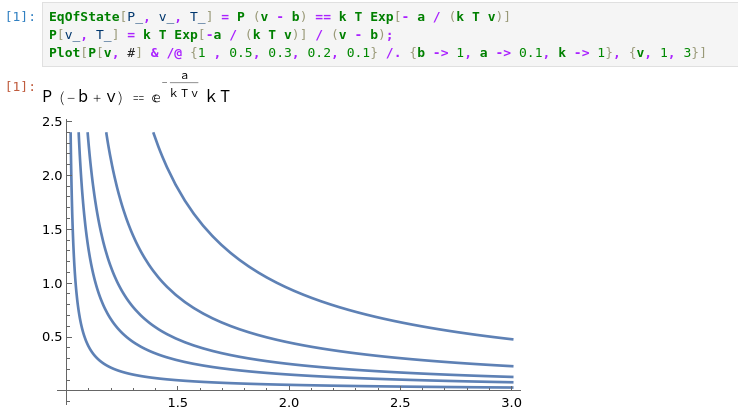
\includegraphics[scale = 0.8]{graphsAndDefinitions.png}
      \end{center}
    \end{figure}

    \begin{enumerate}
      \item
        The critical point is given by the equations: $\frac{\partial P}{\partial v} = \frac{\partial^2 P}{\partial v^2} = 0$, as worked out by the Wolfram engine:
        \begin{figure}[H]
          \begin{center}
            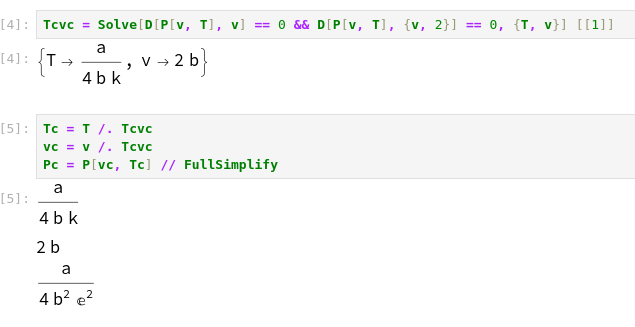
\includegraphics[scale = 0.8]{criticalPoint.png}
          \end{center}
        \end{figure}
        And the equation of state in the reduced variables takes the form:
        \begin{figure}[H]
          \begin{center}
            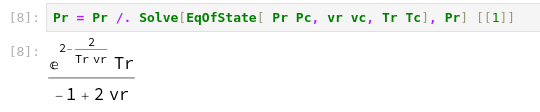
\includegraphics[scale = 0.8]{eqStateRedVar.png}
          \end{center}
        \end{figure}
      \item
        For the $\delta$ critical exponent, the reduced pressure can be expanded in $v_r$ around $v_c = 1$:
        \begin{figure}[H]
          \begin{center}
            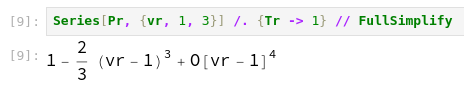
\includegraphics[scale = 0.8]{delta.png}
          \end{center}
        \end{figure}
        For the $\gamma$ critical exponent, the isothermal compressibility $\kappa = -\frac{1}{v}\left(\frac{\partial P}{\partial v}\right)^{-1}$ at the critical volume is expanded in $T$ about $T_c$:
        \begin{figure}[H]
          \begin{center}
            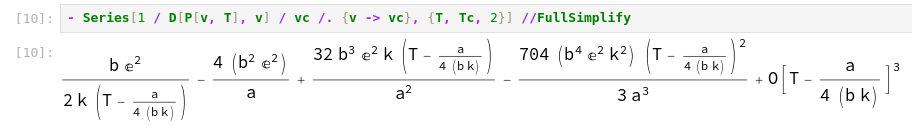
\includegraphics[scale = 0.8]{gamma.png}
          \end{center}
        \end{figure}
      \item
        \begin{figure}[H]
          \begin{center}
            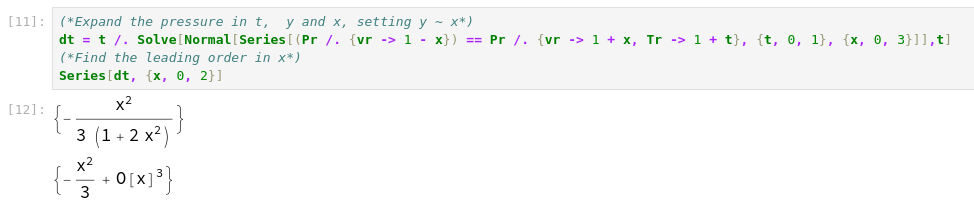
\includegraphics[scale = 0.7]{betaExponent.png}
          \end{center}
        \end{figure}

    \end{enumerate}
\end{enumerate}
\end{document}
